\chapter{Principles and Concepts Characteristic of CouchDB}

\begin{quote}
{\itshape
Django may be built {\bf\it for} the Web, but CouchDB is built {\bf\it of} the Web. I've never seen software that so completely embraces the philosophies behind HTTP. CouchDB makes Django look old-school in the same way that Django makes ASP look outdated.
}

\hspace{1em}---Jacob Kaplan-Moss, Django developer \cite{Kap07}\\
\end{quote}

\noindent
This chapter is intended to give some understanding of main principles and concepts CouchDB is built upon as well as the solution proposed in this work.

One feature that is essential for CouchDB's power, is its table-oriented reporting engine that builds \emph{views} based on dynamically, incrementally generated indexes. The feature is based on the \emph{MapReduce} concept. Because MapReduce and CouchDB views are neither directly relevant to the problem analysis, nor to the proposed solution, their description is omitted. Instead, refer to \cite{DG04} and \cite[p.~53ff]{ASL10}, respectively.


\section{Document-oriented Database}
\label{Document-oriented Database}

CouchDB is a document-oriented database. As opposed to relational databases, document-oriented databases do not store data in tables with uniform sized fields for each record. Instead, each record is stored as a document.\\

\noindent
{\bf Semistructured Data.}
Documents are self-contained units of data and do not have to adhere to a strict separately defined schema. Although a separate schema that places loose constraints on the data may exist, there is no need of a separation between the content's description and the content itself. Because of these properties, documents can be referred to as ``self-describing'' and characterized as \emph{semistructured data} \cite{Bun97}.

There are many forms of data where it would be difficult, or even impossible, to impose a structure on. The most immediate example of data that cannot be constrained by a schema is the World Wide Web \cite{Bun97}. It can be seen as an infinite distributed heterogeneous database. Its primary data format XML, which today is the most popular example of a semistructured data format, is reconciling the concepts of databases and (hypertext) documents \cite{Abi01}.\\

\noindent
{\bf Documents Instead of Rows.}
One of the most fundamental differences between SQL based databases and document-oriented databases is the fundamental unit of data. In SQL, the fundamental unit of data that is dealt with, is the \emph{row}. In a document-oriented database, there are no tables and hence no rows, but \emph{documents} instead. Each document is identified by a unique key.

In the specific case of CouchDB, any documents are JSON documents. Since JSON can express arbitrarily complex data structures, it does not make sense to conceptualize the information in terms of simple rows \cite[p.~14]{Cha09}.


\section{RESTful HTTP Interface}
\label{RESTful HTTP Interface}

Characteristic of CouchDB itself, as well as of systems built on top of CouchDB, is the RESTful HTTP Interface.

Representational State Transfer (REST) is an architectural style for distributed hypermedia systems. An architectural style is a named, coordinated set of architectural constraints \cite[p.~xvi]{Fie00}. Architectures or interfaces conforming to the REST constraints are referred to as being \emph{RESTful}.

REST evolved within the Internet Engineering Taskforce (IETF)\footnote{\url{http://www.ietf.org}} during the development of the Hypertext Transfer Protocol (HTTP/1.0) \cite{rfc1945}, and its extensions HTTP/1.1 \cite{rfc2616} and Uniform Resource Identifiers (URI) \cite{rfc2396}, as an idealized model of how the World Wide Web \emph{should work} \cite[p.~148]{Fie00}. The needs of an internet-scale distributed hypermedia system, like the World Wide Web, are met by enabling processing of actions by intermediaries, dynamic substitutability of components, and the caching and reuse of interactions.

According to Roy Fielding, who introduced and defined REST in 2000 \cite[p.~xvii]{Fie00},
\begin{quote}
REST emphasizes scalability of component interactions, generality of interfaces, independent deployment of components, and intermediary components to reduce interaction latency, enforce security, and encapsulate legacy systems.
\end{quote}

\paragraph{REST Architectural Elements}
Fielding defines a software architecture as ``a configuration of architectural elements---components, connectors, and data---constrained in their relationships in order to achieve a desired set of architectural properties'' \cite[p.~7]{Fie00}. He then defines the terms \emph{configuration}, \emph{component}, \emph{connector}, and \emph{datum} as follows \cite[p.~10ff]{Fie00}:
\begin{quote}
    A component is an abstract unit of software instructions and internal state that provides a transformation of data via its interface.[...]

    A connector is an abstract mechanism that mediates communication, coordination, or cooperation among components.[...]

    A datum is an element of information that is transferred from a component, or received by a component, via a connector.[...]

    A configuration is the structure of architectural relationships among components, connectors, and data during a period of system run-time.
\end{quote}

\begin{table}[h]\small
\begin{tabular}{l l}
\toprule[0.15em]
    {\bf Component}
    &{\bf Modern Web Examples}
\\\midrule[0.15em]
    {origin server}
    &{Apache httpd, CouchDB}
\\\midrule
    {gateway}
    &{CGI, reverse proxy (e.g.\ Squid, CouchDBCP)}
\\\midrule
    {proxy}
    &{Privoxy, Tinyproxy, Transproxy}
\\\midrule
    {user agent}
    &{cURL, Mozilla Firefox, Epiphany}
\\\bottomrule[0.1em]
\end{tabular}
\centering
\caption{REST Components (c.f.\ \cite[p.~96]{Fie00})}
\label{REST_Components}
\end{table}

\begin{table}[h]\small
\begin{tabular}{l l}
\toprule[0.15em]
    {\bf Connector}
    &{\bf Modern Web Examples}
\\\midrule[0.15em]
    {client}
    &{libcurl, lhttpc}
\\\midrule
    {server}
    &{Apache API, Mochiweb}
\\\midrule
    {cache}
    &{browser cache, Akamai cache network}
\\\midrule
    {resolver}
    &{bind (libresolv library), tinydns (djbdns library)}
\\\midrule
    {tunnel}
    &{SOCKS, SSL after HTTP CONNECT}
\\\bottomrule[0.1em]
\end{tabular}
\centering
\caption{REST Connectors (c.f.\ \cite[p.~93]{Fie00})}
\label{REST_Connectors}
\end{table}

\begin{table}[h]\small
\begin{tabular}{l l}
\toprule[0.15em]
    {\bf Data Element}
    &{\bf Modern Web Examples}
\\\midrule[0.15em]
    {resource}
    &{the intended conceptual target of a hypertext reference}
\\\midrule
    {resource identifier}
    &{URL, URN}
\\\midrule
    {representation}
    &{HTML document, JPEG image}
\\\midrule
    {representation metadata}
    &{Last-Modified, Content-Type}
\\\midrule
    {resource metadata}
    &{ETag, Alternates, Vary}
\\\midrule
    {control data}
    &{If-None-Match, Cache-Control}
\\\bottomrule[0.1em]
\end{tabular}
\centering
\caption{REST Data Elements (c.f.\ \cite[p.~88]{Fie00})}
\label{REST_Data_Elements}
\end{table}

The REST style is an abstraction of the architectural elements within a distributed hypermedia system. It focuses on the role of components, the constraints upon their interaction with other components, and their interpretation of significant data elements. The REST constraints define the basis of the web architecture, and thus the essence of the web's behavior as a network-based application \cite[p.~86]{Fie00}.

The tables \ref{REST_Components}, \ref{REST_Connectors}, and \ref{REST_Data_Elements} give a summary of the respective architectural elements.

\paragraph{REST Constraints}
REST places constraints on connector semantics, where in contrast other architectural styles enforcing distributed object access and RPC (Remote Procedure Call) mechanisms (for instance \emph{CORBA}\footnote{Common Object Request Broker Architecture; see \url{http://www.corba.org}}), have focused on component semantics.

The basic REST architectural constraints (cf.\ Sect.~5.1 \cite{Fie00}) are:
\begin{itemize}
	\item {\bf Client-Server} Architectural Style
	\item {\bf Stateless} Communication
	\item Client-side {\bf Cache}
	\item {\bf Uniform Interface} Between Components
	\item {\bf Layered System}.
\end{itemize}

At this point, only the stateless communication constraint will be discussed in detail, as it is strongly related to the other four constraints. A detailed explanation of all REST architectural constraints, as well as a description of the architectural elements and their interplay (i.e.\ architectural views), is given in chapter five of Fielding's dissertation \cite[p.~76ff]{Fie00}. For those who are interested in the subject's practical issues (e.g.\ design and implementation of web services, best practices), the book \emph{RESTful Web Services} \cite{RR07} could be a good source of information. Finally, it should be pointed out that REST itself does not represent an architecture, but rather a set of design criteria (i.e.\ an architectural style). In chapter four of \cite{RR07}, a concrete RESTful architecture, which in contrast to REST, is explicitly tied to the web, is introduced: the \emph{Resource-Oriented Architecture} (ROA).\\

\noindent
{\bf Stateless Communication.}
All REST interactions are stateless; session state is kept entirely on the client. Thus, a request is \emph{self-contained}, i.e., independently of any preceding requests. All of the information that is necessary for a connector to understand a request, is contained in the request.

According to \cite[p.~93]{Fie00}, this restriction accomplishes four functions:
\begin{quote}
1) it removes any need for the connectors to retain application state between requests, thus reducing consumption of physical resources and improving scalability;

2) it allows interactions to be processed in parallel without requiring that the processing mechanism understand the interaction semantics;

3) it allows an intermediary to view and understand a request in isolation, which may be necessary when services are dynamically rearranged; and,

4) it forces all of the information that might factor into the reusability of a cached response to be present in each request.
\end{quote}

In a nutshell, stateless communication induces the properties of \emph{visibility}, \emph{reliability}, and \emph{scalability} \cite[p.~79]{Fie00}. Visibility is facilitated, because a monitoring system does not have to look beyond a single request datum in order to determine the full nature of the request. Reliability is facilitated, because statelessness eases the task of recovering from partial failures \cite{KWWW94}. Scalability is facilitated, because not having to store state between requests allows the server component to quickly free resources, and further simplifies implementation, as there is no need to manage resource usage across requests.

Furthermore, because stateless communication allows each interaction to be independent of the others, there is no need for an awareness of the overall component topology, which would be an impossible task for an Internet-scale architecture, anyway. Components can either act as a destination or as a intermediary, determined dynamically by the target of each request. Therefore, RESTful web services may be implemented using a complex hierarchy of intermediaries and multiple distributed origin servers \cite[p.~99]{Fie00}.\\

\noindent
{\bf Example: CouchDB's RESTful HTTP Interface.}
CouchDB's REST API features basically three HTTP methods: {\tt GET}, {\tt PUT}, and {\tt DELETE}. As an example, if a request's target is a document, the individual methods feature the following semantics:

\begin{itemize}
	\item {\tt GET}: retrieve a document or document attachment.
	\item {\tt PUT}: create or update a document or document attachment.
	\item {\tt DELETE}: delete a document.
\end{itemize}  

The {\tt POST} method, amongst other things, is used to trigger replication. However, it cannot be spoken of as a part of the REST API, because it is not corresponding to REST, but to an RPC style instead \cite[p.~44]{ASL10}.

A detailed hands-on introduction to CouchDB's API can be found in chapter four of \cite{ASL10}, whereas the exhaustive API reference can be retrieved online\footnote{\url{http://wiki.apache.org/couchdb/Reference}}.


\section{Multiversion Concurrency Control}
\label{Multiversion Concurrency Control}

In this section the terms \emph{Concurrency Control} and \emph{Multiversion Concurrency Control}, as well as the respective correctness criteria, \emph{serializability} and \emph{one-copy serializability}, are explained. The goal is to give an idea of those concepts, to be able to understand the principles behind CouchDB's Multiversion Concurrency Control implementation. For exhaustive definitions and descriptions of those concepts see \cite{Pap79}, \cite{BG81}, and \cite{BG83}.\\

\noindent
{\bf Transactions.}
The unit of data processing in a distributed system is the \emph{transaction}. A transaction is a portion of a program that issues reads and writes to a database system (DBS). For concreteness, one can assume that each transaction is a process, and each data item is managed by a separate process. (However, the assumption is not required) \cite{BG82}. In addition, it is assumed that a transaction transforms a consistent state into a new consistent state.

A transaction's outcome can be that it has either \emph{aborted}, because an operation was rejected by the DBS for some reason, or that it has \emph{commited}, and all operations were executed successfully. In case of an abort, every involved data item is left in the same state as before the transaction. In short, a transaction appears to execute either completely (it is said to \emph{commit}) or not at all (it is said to \emph{abort}). This property is referred to as \emph{failure atomicity} \cite[p.~242f]{GR06}.\\

\noindent
{\bf Concurrency Control's Purpose.}
Concurrency Control (CC) solves the problem of synchronizing concurrently executing transactions on a shared database. When transactions execute concurrently, the interleaved execution of their reads and writes by the DBS can produce undesirable results. CC is the activity of avoiding such undesirable results \cite{BG82}.

According to \cite{BG81}, ``The correctness of a concurrency control algorithm is defined relative to users' expectations regarding transaction execution'', and there are two correctness criteria, whose realization is CC's  principal issue:
\begin{quote}
(1) users expect that each transaction submitted to the system will eventually be executed;

(2) users expect the computation performed by each transaction to be the same whether it executes alone in a dedicated system or in parallel with other transactions in a multiprogrammed system.
\end{quote}

\vspace{0.5em}
\noindent
{\bf Serializability.}
In accordance with the just illustrated correctness criteria, the goal of CC is to guarantee \emph{serializable} execution of transactions. Thus, the notion of correctness in this context is that of \emph{serializability}, which is attained by controlling the order in which reads and writes are processed \cite{Pap79} \cite{BG83}.

In \cite{BG81}, serializability has been described as follows:
\begin{quote}
Let $E$ denote an execution of transactions $T_1, ..., T_n$. $E$ is a serial execution if no transactions execute concurrently in $E$; that is, each transaction is executed to completion before the next one begins. [...] An execution is serializable if it is computationally equivalent to a serial execution, that is, if it produces the same output and has the same effect on the database as some serial execution.
\end{quote}

\paragraph{Single-version Concurrency Control}
When dealing with concurrent data operations, a DBS must, in order to preserve data consistency, prevent the modification of data items while being read, and vice versa, must prevent data items from being read while being modified. In single-version DBSs, this is achieved by maintaining \emph{locks} of the respective data items. Transactions trying to modify data items that are concurrently read by different transactions are blocked, until the locks on the respective data items are released. As a consequence, \emph{deadlocks} may occur. For an example, take two transactions, each with a lock whose release the other transaction is waiting for. This problem can be handled by either prevention, or detection and elimination (see \cite{BG81}).

Another problem becomes evident when a transaction has modified data items and, for some reason, fails to complete. In this case, data items are likely to be inconsistent. However, as stated before, an essential property of transactions is failure atomicity. To preserve this property, a transaction \emph{rollback} mechanism has to be established. In the case of a transaction abort, the data items' state before the transaction is restored by the rollback mechanism. In order to guarantee that rollbacks can be performed at any time (imagine a database recovery, succeeding a failure that occurred while transactions were being executed), the rollback mechanism has to be able to retrieve all required data from a durable \emph{transaction log}, which is maintained by a \emph{log manager} (see \cite[p.~493ff]{GR92}).

\paragraph{Multiversion Concurrency Control}
According to \cite{Sil82}, the concept of Multiversion Concurrency Control (MVCC) has been used as early as 1973 in a version of the Honeywell FMS system \cite{Hon73}, and was formalized in \cite{SLR76}. The first description of a MVCC algorithm that is known of, is Reed's multiversion timestamping algorithm \cite{Ree78}. However, the term ``Multiversion Concurrency Control'' itself initially appeared later, e.g.\ in \cite{Sil82}.

In a multiversion DBS, each write on a data item $x$, produces a new copy (i.e.\ a version) of $x$. Versions of $x$ are denoted by $x_i, x_j, ...$, where the subscript is the index of the transaction that wrote the version. Operations on versions are denoted $r_i[x_j]$ and $w_i[x_i]$. For each read on $x$, the DBS selects one of the versions of $x$ to be read. To execute a transaction $T_i$, a multiversion DBS must \emph{translate} the transaction's ``data item operations'' into ``version operations''. This \emph{translation} can be formalized by a function, which maps each write operation $w_i[x]$ into $w_i[x_i]$ and each read operation $r_i[x]$ into $r_i[x_j]$ for some $j$.

Since writes do not overwrite each other, and since reads can read any version, the DBS has more flexibility in controlling the order of reads and writes. In contrast to single-version CC, one-copy serializability (see below) can be achieved without locking when (logical) timestamps are used. Because it is not necessary for a read access to a data item to lock out writes to the data item, and vice versa, writes do not need to block reads. Therefore, MVCC can allow more concurrency than single-version CC \cite[p.~158]{Ree78} \cite{BG83}.\\

\noindent
{\bf One-Copy Serializability.}
In contrast to a single-version database, where CC correctness only depends on the order in which reads and writes are processed, in a multiversion database it depends on the translation as well as the order. The corresponding correctness condition for MVCC algorithms is \emph{one-copy serializability}: an execution of transactions in a multiversion database is one-copy serializable, if it is equivalent to a serial execution of the same transactions in a single-version database \cite{BG83}.\\

\noindent
{\bf Multiversion Timestamping.}
The earliest MVCC algorithm that is known of is Reed's multiversion timestamping algorithm \cite{Ree78}.

When it begins executing, each transaction is assigned a unique \emph{timestamp} $TS(i)$, which tells the \emph{logical time} at which the transaction began. The timestamps are assigned by a \emph{logical clock} (see \cite{Lam78}), and hence are strictly increasing. Each read/write operation carries a timestamp (that of the transaction that issued it), and each version carries the timestamp of the transaction that wrote it.

Operations are basically processed first-come-first-served, but the translation from data item operations to version operations makes it appear as if they were processed in timestamp order.

According to \cite{BG83}, the algorithm works as follows:
\begin{quote}
  \begin{enumerate}[(1)]
    \item $r_i[x]$ is translated into $r_i[x_k]$, where $x_k$ is the version of $x$ with largest timestamp $\leq$ $TS(i)$.

    \item $w_i[x]$ has two cases. If the DBS has already processed $r_j[x_k]$ such that $TS(k) < TS(i) < TS(j)$, then $w_i[x]$ is \emph{rejected}. Otherwise $w_i[x]$ is translated into $w_i[x_i]$. Intuitively, $w_i[x]$ is rejected if it would invalidate $r_j[x_k]$.
  \end{enumerate}
\end{quote}

\vspace{0.5em}
\noindent
{\bf Example: CouchDB's MVCC Implementation.}
\begin{figure}[ht]
	{\flushleft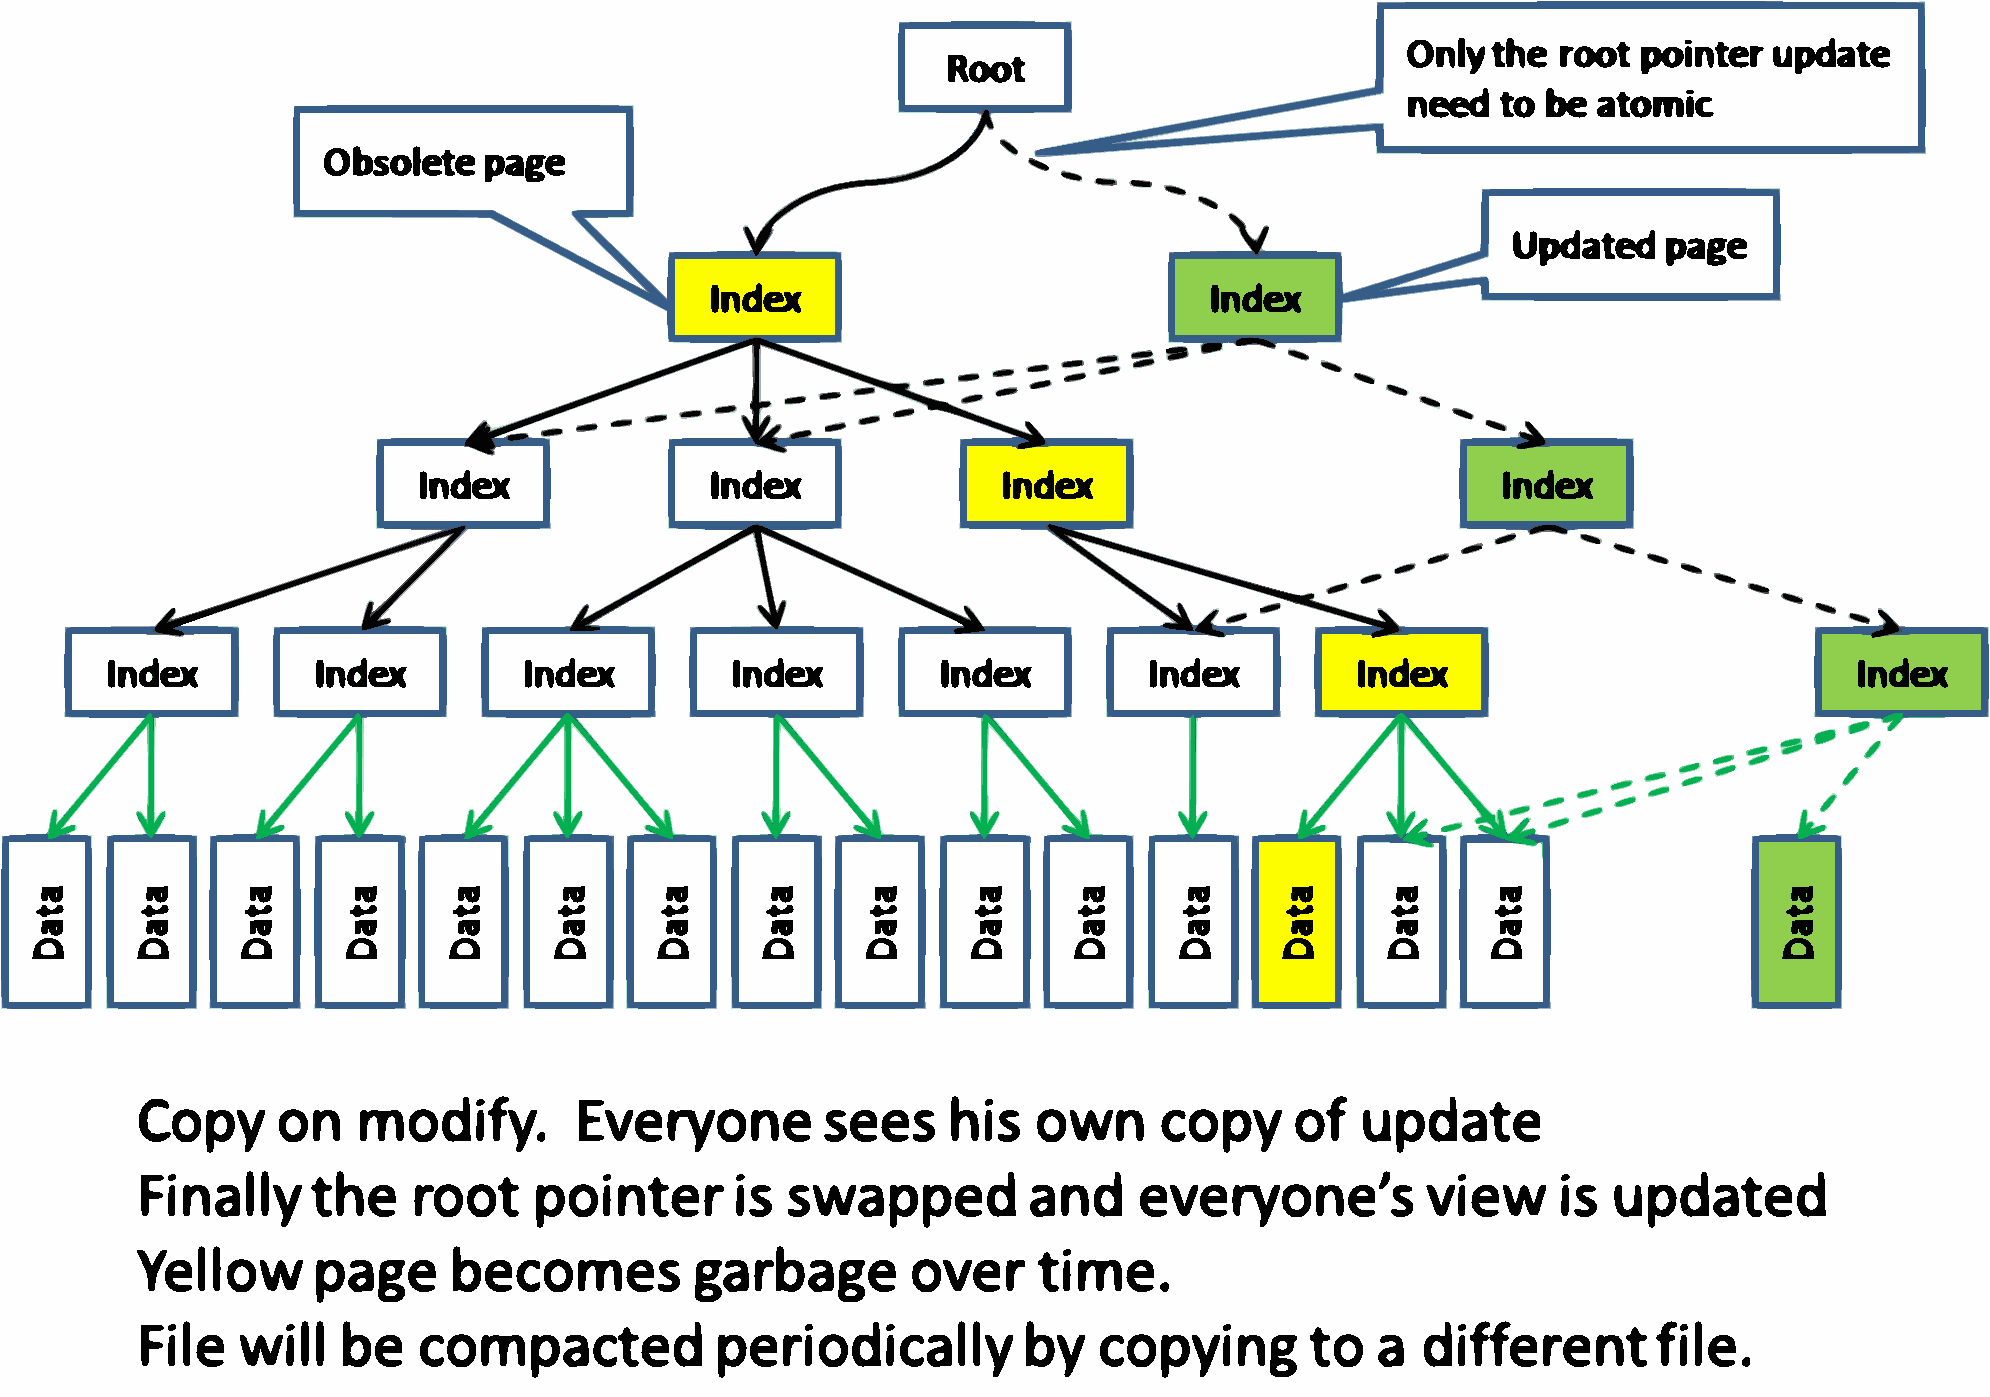
\includegraphics[width=\textwidth]{figures/MVCC}}
	\caption{CouchDB's MVCC index structure. Courtesy of Ricky Ho \cite{Ho09}.}
	\label{Ho09}
\end{figure}
CouchDB's MVCC mechanism ensures that, in case somebody else made a change unbeknownst to the updating client, its update will not be accepted. In order to update a document (that includes its deletion), the document's latest revision (i.e.\ version) number has to be specified in the respective request's query parameter {\tt rev}. (The concept behind CouchDB's revision numbers is explained comprehensively in section \ref{Replication and Conflict Management}.) The reason for that constraint is that it prevents clients from updating data they did not know existed. Simplified, it can be said that ``whoever saves a change to a document first, wins'' \cite[p.~39]{ASL10}.

To understand CouchDB's MVCC implementation, it is helpful to look at CouchDB's index structure. The data structure that is used to index documents and views is the $B^+$-tree.\footnote{Regarding the $B^+$-tree data structure, it is referred to \cite{Bay08} and \cite{Com79}.} For each database and for each view index, one $B^+$-tree is used. CouchDB's $B^+$-tree implementation features an append-only design. As illustrated in figure \ref{Ho09}, write-locks are only needed for one simple operation, namely for an update of the index's root pointer. Read-locks are not necessary at all.

Writes need to be serialized, so that for any single database only one write operation is allowed at any point in time. The reason is that for every write operation in a database, the $B^+$-tree's root node has to be rewritten in the database file. In doing so, like the $B^+$-tree, the database file is append-only as well. Old portions of the database file will never change, and every old $B^+$-tree root, in case that there are still references to it, will point to a consistent snapshot of the database.

Following from the described design, there can be any number of read operations at any given time, and each read operation is guaranteed a consistent view of the database.

For more details, e.g.\ on how failure atomicity and local data consistency are guaranteed at any time, see \cite[p.~233ff]{ASL10}.


\section{Replication and Conflict Management}
\label{Replication and Conflict Management}

{\bf Replication.}
CouchDB has a peer-to-peer replication feature that allows for uni- and bi-directional replication of any database changes. So it is possible to have several synchronized copies of the same database arranged in a decentralized fashion. Neither coordination of read/write operations nor central infrastructure is needed. Thus, the peer-to-peer replication feature allows for the creation of decentralized, eventual consistent CouchDB clusters.

The replication process, which is started by an HTTP {\tt POST} request, works incrementally. Only documents updated since the last replication are examined, and for each updated document only the changes are replicated. If replication fails, e.g.\ due to network problems or crash, the next replication restarts at the same document where it left off.

Replication can be triggered in two different modes: in pull mode it will be executed once, so that only the current changes will be replicated, in push mode not only the current changes but also future changes will be replicated continuously.

Furthermore, replication can be filtered by custom filter functions written in JavaScript or Erlang, so that only particular documents or those meeting specific criteria are replicated \cite[p.~149ff]{ASL10} \cite{Apa10}.\\

\noindent
{\bf Conflict Management.}
In CouchDB, conflicts are treated as a common state, not an exceptional one. Consequently, any number of conflicting document versions may exist in a database concurrently.

Each version (also referred to as \emph{revision}) of a CouchDB document has a deterministic unique revision history, which basically is an ordered list of the actual and all past revision numbers, stored in the document metadata. A particular document version can be retrieved by specifying its revision number in the respective HTTP {\tt GET} request as a value of the URL query parameter {\tt rev}. If the query parameter is not specified, the latest version is retrieved.

A conflict may occur when a document is replicated to a database. In particular, it occurs when two or more documents with the same identifier have a revision history that is of the same length, but the documents' revision histories or data differ. In this case, all conflicting document versions are stored, and each version is marked with a specific \emph{conflicts} flag.

In the presence of conflicts, some order between conflicting versions of a document needs to be established to decide over ``winning'' and ``losing'' versions. Except that only winning versions can appear in views, losing versions are just like any other version. They can be retrieved by specifying the revision number as a query parameter value and are also replicated.

A deterministic decentralized conflict management mechanism is important in a distributed system with redundant instances of the same database. Independently of the other instances' state or some other shared state (like e.g.\ chronological time), each instance is able to make deterministic decisions about the different versions' order.

When distributed update conflicts occur, all database replicas see the same winning revision, and each has the opportunity to resolve the conflict. Resolving conflicts can be done manually or, depending on the nature of the data and the conflict, by automated agents. Decentralized conflict resolution is possible while maintaining single document database semantics \cite{Apa10}.\\

\noindent
{\bf Deterministic Revision Numbers.} Revision numbers consist of an integer followed by a dash and a hash code: e.g.\ {\tt 3-5d0319b075a21b095719bc561def7122}. The integer is incremented for each new document revision and starts with the value $1$. The hash code is a md5 hash code over a set of document properties: the JSON body and some metadata fields. When there are conflicts, revision numbers are compared in ASCII sort order and the one with the highest ASCII values wins. Documents with the same content and revision history (and practically only those ones) have the same revision number and will not create any conflicts \cite[p.~153ff]{ASL10}.

A desired effect of this scheme is that it is deterministic and there is no need for shared state. This is also true for a distributed system, where for one version of a document there can be as many conflicting versions as the number of distributed nodes minus one. Take as an example that every node replicates its changes to every other node. Every node can make its conflict decision independently of the other nodes, without any shared state. Eventually (once each node has replicated its changes to every other node), all nodes will agree and expose the same view.
